\documentclass[11pt,a4paper]{article}

\usepackage[margin=20mm,headheight=15pt]{geometry}

\usepackage{longtable,booktabs,array,hyperref,xcolor,tikz,fancyhdr}

\usepackage{fontspec,xeCJK}

\setmainfont[Ligatures=TeXOff]{Times New Roman}

\setsansfont[Ligatures=TeXOff]{Times New Roman}

\setmonofont[Ligatures=TeXOff,WordSpace={1,1,1}]{Times New Roman}

\setCJKmainfont{Noto Serif CJK SC}

\setCJKsansfont{Noto Serif CJK SC}

\setCJKmonofont{Noto Serif CJK SC}

\newfontfamily\vulcanmathsymbols{Noto Serif CJK SC}

\XeTeXgenerateactualtext=1

\definecolor{vulcan}{HTML}{BB3E23}

\pgfdeclarelayer{connections}\pgfdeclarelayer{edge labels}\pgfsetlayers{connections,main,edge labels}

\hypersetup{hidelinks}

\newcolumntype{L}[1]{>{\raggedright\arraybackslash}p{#1}}

\setlength{\emergencystretch}{5em}\tolerance=2000\hbadness=10000

\setlength{\parindent}{0pt}\setlength{\parskip}{5pt}

\pagestyle{fancy}\fancyhf{}\fancyhead[L]{\small\sffamily\textbf{VULCAN SILICON ENGINEERING}}

\fancyhead[R]{\small\sffamily Technical Design, Quartus STA \& FPGA Verification Report}\fancyfoot[C]{\small\sffamily Page \thepage}

\begin{document}

{\footnotesize\sffamily\textcolor{vulcan}{\textbf{VULCAN AUTONOMOUS CHIP DESIGN \& HARDWARE SIGNOFF SERIES \hfill DOCUMENT CLASS: ENGINEERING VERIFICATION REPORT}}\par}

\vspace{2pt}\textcolor{vulcan}{\rule{\textwidth}{1.2pt}}\vspace{4pt}

{\sffamily\LARGE\raggedright\textbf{BILLET-T2: Runtime-Configurable FFT/\allowbreak{}IFFT RTL IP}\par}

\vspace{4pt}

{\footnotesize\sffamily\renewcommand{\arraystretch}{1.22}\begin{tabular}{@{}L{0.22\textwidth}L{0.74\textwidth}@{}}\toprule\textbf{Author \& Contact} & Sufeng Guo (\allowbreak{}sufeng\_\allowbreak{}guo@smail.nju.edu.cn,\allowbreak{} v-sufengguo@microsoft.com)\allowbreak{}\\\textbf{Target Platform} & Intel Arria 10 GX (\texttt{10AX115N3F40E2SG}) \textemdash{} Microsoft Catapult Longs Peak (Bedrock 2.1)\\\textbf{Verification Stack} & Icarus Verilog 12.0 $\cdot$ Yosys 0.33 $\cdot$ Intel Quartus Prime 17.1 TimeQuest STA $\cdot$ PCIe Gen3x8 HIL\\\textbf{Release Timestamp} & 2026-10-19 23:40 UTC+\allowbreak{}8 (\allowbreak{}Beijing Time)\allowbreak{}\\\bottomrule\end{tabular}\par}

\vspace{4pt}

\begin{abstract}\noindent 

BILLET-T2 is a synthesizable SystemVerilog transform engine supporting runtime-selected 16-,\allowbreak{} 32-,\allowbreak{} 64-,\allowbreak{} 128- and 256-point complex FFTs and IFFTs. A single iterative radix-2 datapath provides fixed,\allowbreak{} programmable and block floating-point stage scaling,\allowbreak{} natural-order input/\allowbreak{}output and frame-level exponent metadata.


Independent RTL simulation checked 479 main-matrix frames across 1,\allowbreak{}209,\allowbreak{}230 cycles. Separate simulations established bit-exact BILLET-T1 compatibility for twelve 256-point forward/\allowbreak{}fixed frames. Fifteen FFT-to-IFFT reconstructions achieved worst component error of 5 input LSB and worst complex-sample RMS error of 2.003902 LSB,\allowbreak{} below the respective 32- and 8-LSB limits. BFP reduced exponent-rescaled spectral error for the specified impulse demonstration at every supported length. Generic synthesis retained substantive arithmetic and storage without inferred latches or unresolved modules. These results establish RTL-IP functionality and generic synthesizability,\allowbreak{} not physical implementation performance. [\allowbreak{}E023,\allowbreak{} E024]\allowbreak{}


\end{abstract}

\section{Architecture and design rationale}

The parameterless billet\_\allowbreak{}t2\_\allowbreak{}top instantiates the bit-reversal,\allowbreak{} twiddle-ROM,\allowbreak{} butterfly and BFP-scaler modules directly. It owns configuration,\allowbreak{} scheduling,\allowbreak{} memories,\allowbreak{} diagnostics and output holding registers. Bit-reversed loading permits natural-order radix-2 DIT results. Each stage computes all raw butterflies before normalization,\allowbreak{} preserving information until the complete-stage BFP decision is available. This deliberately trades scratch storage and latency for a simple shared datapath with deterministic scheduling. The two banks contain 17,\allowbreak{}408 logical bits; physical memory inference is target-dependent. Blocks below are ordered row-major for a three-column diagram. [\allowbreak{}E001–E007]\allowbreak{}

\begin{center}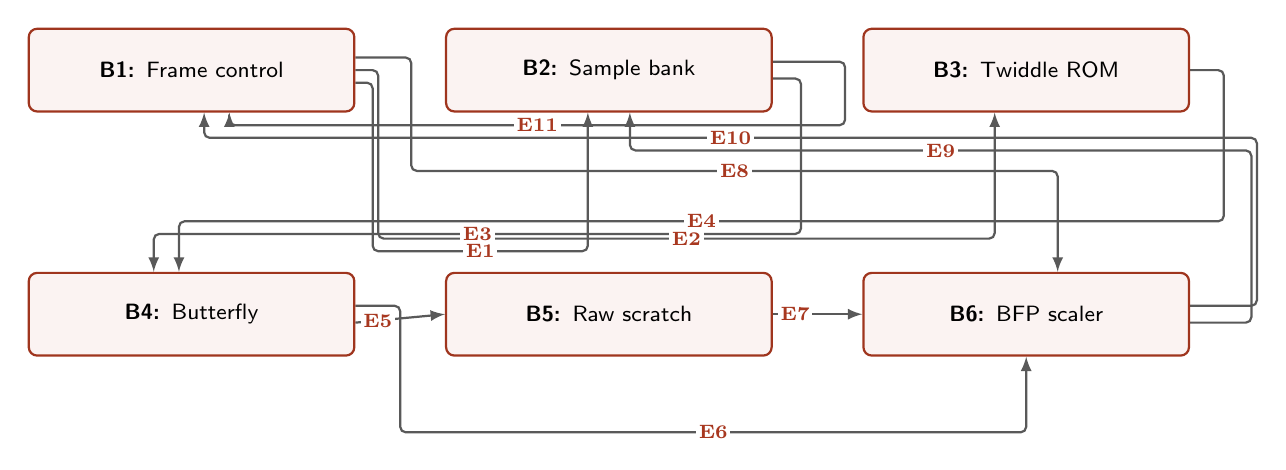
\begin{tikzpicture}[every node/.style={font=\footnotesize\sffamily},>=latex]

\node[draw=vulcan!85!black,thick,rounded corners=3pt,fill=vulcan!6,text width=3.9cm,minimum height=1.05cm,align=center] (b0) at (0.0,0.0) {\textbf{B1:} Frame control};

\node[draw=vulcan!85!black,thick,rounded corners=3pt,fill=vulcan!6,text width=3.9cm,minimum height=1.05cm,align=center] (b1) at (5.3,0.0) {\textbf{B2:} Sample bank};

\node[draw=vulcan!85!black,thick,rounded corners=3pt,fill=vulcan!6,text width=3.9cm,minimum height=1.05cm,align=center] (b2) at (10.6,0.0) {\textbf{B3:} Twiddle ROM};

\node[draw=vulcan!85!black,thick,rounded corners=3pt,fill=vulcan!6,text width=3.9cm,minimum height=1.05cm,align=center] (b3) at (0.0,-3.1) {\textbf{B4:} Butterfly};

\node[draw=vulcan!85!black,thick,rounded corners=3pt,fill=vulcan!6,text width=3.9cm,minimum height=1.05cm,align=center] (b4) at (5.3,-3.1) {\textbf{B5:} Raw scratch};

\node[draw=vulcan!85!black,thick,rounded corners=3pt,fill=vulcan!6,text width=3.9cm,minimum height=1.05cm,align=center] (b5) at (10.6,-3.1) {\textbf{B6:} BFP scaler};

\begin{pgfonlayer}{connections}

\draw[->,thick,black!65,rounded corners=2pt] ([yshift=-0.160cm]b0.east) -- (2.300,-0.160) -- (2.300,-2.300) -- coordinate[midway] (e0) (5.033,-2.300) -- ([xshift=-0.267cm]b1.south);

\draw[->,thick,black!65,rounded corners=2pt] ([yshift=0.000cm]b0.east) -- (2.370,0.000) -- (2.370,-2.140) -- coordinate[midway] (e1) (10.200,-2.140) -- ([xshift=-0.400cm]b2.south);

\draw[->,thick,black!65,rounded corners=2pt] ([yshift=-0.107cm]b1.east) -- (7.740,-0.107) -- (7.740,-2.080) -- coordinate[midway] (e2) (-0.480,-2.080) -- ([xshift=-0.480cm]b3.north);

\draw[->,thick,black!65,rounded corners=2pt] ([yshift=0.000cm]b2.east) -- (13.110,0.000) -- (13.110,-1.920) -- coordinate[midway] (e3) (-0.160,-1.920) -- ([xshift=-0.160cm]b3.north);

\draw[->,thick,black!65] ([yshift=-0.107cm]b3.east) -- coordinate[pos=0.25] (e4) ([yshift=0.000cm]b4.west);

\draw[->,thick,black!65,rounded corners=2pt] ([yshift=0.107cm]b3.east) -- (2.650,-2.993) -- (2.650,-4.600) -- coordinate[midway] (e5) (10.600,-4.600) -- ([xshift=0.000cm]b5.south);

\draw[->,thick,black!65] ([yshift=0.000cm]b4.east) -- coordinate[pos=0.25] (e6) ([yshift=0.000cm]b5.west);

\draw[->,thick,black!65,rounded corners=2pt] ([yshift=0.160cm]b0.east) -- (2.790,0.160) -- (2.790,-1.280) -- coordinate[midway] (e7) (11.000,-1.280) -- ([xshift=0.400cm]b5.north);

\draw[->,thick,black!65,rounded corners=2pt] ([yshift=-0.107cm]b5.east) -- (13.460,-3.207) -- (13.460,-1.020) -- coordinate[midway] (e8) (5.567,-1.020) -- ([xshift=0.267cm]b1.south);

\draw[->,thick,black!65,rounded corners=2pt] ([yshift=0.107cm]b5.east) -- (13.530,-2.993) -- (13.530,-0.860) -- coordinate[midway] (e9) (0.160,-0.860) -- ([xshift=0.160cm]b0.south);

\draw[->,thick,black!65,rounded corners=2pt] ([yshift=0.107cm]b1.east) -- (8.300,0.107) -- (8.300,-0.700) -- coordinate[midway] (e10) (0.480,-0.700) -- ([xshift=0.480cm]b0.south);

\end{pgfonlayer}

\begin{pgfonlayer}{edge labels}

\node[fill=white,inner sep=1pt,font=\scriptsize\bfseries,text=vulcan!90!black] at (e0) {E1};

\node[fill=white,inner sep=1pt,font=\scriptsize\bfseries,text=vulcan!90!black] at (e1) {E2};

\node[fill=white,inner sep=1pt,font=\scriptsize\bfseries,text=vulcan!90!black] at (e2) {E3};

\node[fill=white,inner sep=1pt,font=\scriptsize\bfseries,text=vulcan!90!black] at (e3) {E4};

\node[fill=white,inner sep=1pt,font=\scriptsize\bfseries,text=vulcan!90!black] at (e4) {E5};

\node[fill=white,inner sep=1pt,font=\scriptsize\bfseries,text=vulcan!90!black] at (e5) {E6};

\node[fill=white,inner sep=1pt,font=\scriptsize\bfseries,text=vulcan!90!black] at (e6) {E7};

\node[fill=white,inner sep=1pt,font=\scriptsize\bfseries,text=vulcan!90!black] at (e7) {E8};

\node[fill=white,inner sep=1pt,font=\scriptsize\bfseries,text=vulcan!90!black] at (e8) {E9};

\node[fill=white,inner sep=1pt,font=\scriptsize\bfseries,text=vulcan!90!black] at (e9) {E10};

\node[fill=white,inner sep=1pt,font=\scriptsize\bfseries,text=vulcan!90!black] at (e10) {E11};

\end{pgfonlayer}

\end{tikzpicture}\par

{\small\textbf{Figure 1:} Top-level microarchitectural functional block map and directed inter-module bus topology.}\end{center}

{\small\renewcommand{\arraystretch}{1.18}\begin{longtable}{@{}L{0.24\textwidth}L{0.7\textwidth}@{}}\toprule

\textbf{Block} & \textbf{Responsibility}\\\midrule\endhead

B1: Frame control & Top-level handshake,\allowbreak{} latched configuration,\allowbreak{} counters,\allowbreak{} bit-reversal instance,\allowbreak{} stage scheduling,\allowbreak{} output holding registers and cumulative diagnostics.\\[3pt]

B2: Sample bank & One 256-by-32-bit bank stores complex signed-16 samples,\allowbreak{} normalized stage results and final natural-order bins.\\[3pt]

B3: Twiddle ROM & Canonical 256-grid forward constants,\allowbreak{} addressed over 0–127; signed-17-bit outputs support exact inverse conjugation.\\[3pt]

B4: Butterfly & One time-multiplexed complex butterfly forms full-width products and four unclipped signed-18-bit raw components.\\[3pt]

B5: Raw scratch & One 256-by-36-bit bank preserves every complex raw stage result before any stage normalization.\\[3pt]

B6: BFP scaler & Accumulates stage headroom,\allowbreak{} selects zero/\allowbreak{}one-bit scaling,\allowbreak{} saturates normalized components and accumulates the frame exponent.\\[3pt]

\bottomrule\end{longtable}}

{\small\renewcommand{\arraystretch}{1.18}\begin{longtable}{@{}L{0.24\textwidth}L{0.7\textwidth}@{}}\toprule

\textbf{Directed relationship} & \textbf{Meaning}\\\midrule\endhead

E1: B1 to B2 & Bit-reversed input writes and scheduled bank access\\[3pt]

E2: B1 to B3 & Stage twiddle address and latched direction\\[3pt]

E3: B2 to B4 & Registered operand pair\\[3pt]

E4: B3 to B4 & Quantized complex coefficient\\[3pt]

E5: B4 to B5 & Two raw complex writes per butterfly\\[3pt]

E6: B4 to B6 & Four-component headroom observation\\[3pt]

E7: B5 to B6 & Registered normalization operand\\[3pt]

E8: B1 to B6 & Frame/\allowbreak{}stage controls and scaling configuration\\[3pt]

E9: B6 to B2 & Scaled,\allowbreak{} saturated normalization writeback\\[3pt]

E10: B6 to B1 & Exponent and component saturation increment\\[3pt]

E11: B2 to B1 & Final-bin fetch into output holding register\\[3pt]

\bottomrule\end{longtable}}

\section{Interfaces and configuration}

{\small\renewcommand{\arraystretch}{1.18}\begin{longtable}{@{}L{0.2\textwidth}L{0.12\textwidth}L{0.1\textwidth}L{0.48\textwidth}@{}}\toprule

\textbf{Signal /\allowbreak{} group} & \textbf{Direction} & \textbf{Width} & \textbf{Contract}\\\midrule\endhead

clk,\allowbreak{} rst\_\allowbreak{}n & Input & 1 bit each & Rising-edge clock and asynchronous active-low reset. Every public output is zero while reset is asserted.\\[3pt]

in\_\allowbreak{}valid,\allowbreak{} in\_\allowbreak{}last,\allowbreak{} in\_\allowbreak{}ready & Input: in\_\allowbreak{}valid,\allowbreak{} in\_\allowbreak{}last; output: in\_\allowbreak{}ready & 1 bit each & Accept a sample only on a rising edge with valid and ready. in\_\allowbreak{}last is advisory; exactly N accepted samples define a frame.\\[3pt]

in\_\allowbreak{}re,\allowbreak{} in\_\allowbreak{}im & Input & Signed 16 bits each & Natural-order complex Q1.15 integer codes,\allowbreak{} representing each component divided by 32768.\\[3pt]

cfg\_\allowbreak{}log2\_\allowbreak{}n,\allowbreak{} cfg\_\allowbreak{}ifft & Input & 4 bits; 1 bit & Length exponent 4–8; direction 0 selects forward FFT and 1 selects conjugated-twiddle,\allowbreak{} unnormalized IFFT.\\[3pt]

cfg\_\allowbreak{}scale\_\allowbreak{}mode,\allowbreak{} cfg\_\allowbreak{}stage\_\allowbreak{}shift\_\allowbreak{}mask & Input & 2 bits; 8 bits & Modes 0=\allowbreak{}fixed,\allowbreak{} 1=\allowbreak{}programmable,\allowbreak{} 2=\allowbreak{}BFP; mode 3 is invalid. Mask bit s controls active stage s only in mode 1.\\[3pt]

out\_\allowbreak{}valid,\allowbreak{} out\_\allowbreak{}ready,\allowbreak{} out\_\allowbreak{}last & Output: out\_\allowbreak{}valid,\allowbreak{} out\_\allowbreak{}last; input: out\_\allowbreak{}ready & 1 bit each & Valid/\allowbreak{}ready output transfers. Last accompanies only valid bin N{\vulcanmathsymbols −}1. Payload and metadata remain stable throughout a stall.\\[3pt]

out\_\allowbreak{}re,\allowbreak{} out\_\allowbreak{}im,\allowbreak{} out\_\allowbreak{}bin\_\allowbreak{}idx,\allowbreak{} out\_\allowbreak{}block\_\allowbreak{}exp & Output & Signed 16 bits each; 8 bits; 4 bits & Natural-order complex result,\allowbreak{} bin index and total stage-shift exponent E. Exponent is identical for every bin in a frame. All these fields are zero when out\_\allowbreak{}valid is zero.\\[3pt]

frame\_\allowbreak{}done,\allowbreak{} cfg\_\allowbreak{}error & Output & 1 bit each & Done pulses for one cycle immediately after final output acceptance. Error identifies invalid live configuration only while idle; it is zero during active frames and reset.\\[3pt]

overflow\_\allowbreak{}flag,\allowbreak{} saturation\_\allowbreak{}count & Output & 1 bit; 32 bits & Reset-only sticky overflow and cumulative clamped-component count. Counter saturates at 0xffffffff rather than wrapping.\\[3pt]

\bottomrule\end{longtable}}

{\small\renewcommand{\arraystretch}{1.18}\begin{longtable}{@{}L{0.23\textwidth}L{0.12\textwidth}L{0.57\textwidth}@{}}\toprule

\textbf{Parameter} & \textbf{Default} & \textbf{Meaning /\allowbreak{} supported values}\\\midrule\endhead

Public elaboration parameters & None & The top and four subordinate modules expose no parameters. MAX\_\allowbreak{}N=\allowbreak{}256 and signed sample width=\allowbreak{}16 are fixed.\\[3pt]

Runtime length and direction & No public default & Drive legal configuration before the first transfer: cfg\_\allowbreak{}log2\_\allowbreak{}n {\vulcanmathsymbols ∈} \{4,\allowbreak{}5,\allowbreak{}6,\allowbreak{}7,\allowbreak{}8\},\allowbreak{} cfg\_\allowbreak{}ifft {\vulcanmathsymbols ∈} \{0,\allowbreak{}1\}. Internal reset values do not constitute a usable frame configuration.\\[3pt]

Runtime scaling & No public default & cfg\_\allowbreak{}scale\_\allowbreak{}mode {\vulcanmathsymbols ∈} \{0,\allowbreak{}1,\allowbreak{}2\}; stage mask is any 8-bit value. Bits above log2(\allowbreak{}N)\allowbreak{}{\vulcanmathsymbols −}1 are ignored.\\[3pt]

\bottomrule\end{longtable}}

\section{Behavior and corner cases}

\subsection{Configuration and frame ownership}

The first accepted sample latches the complete configuration. Later configuration changes are ignored through final output acceptance,\allowbreak{} including during loading. Invalid idle configuration suppresses ready and asserts cfg\_\allowbreak{}error. There is one live frame,\allowbreak{} with no overlap; the next frame can first transfer on the edge following the previous final output handshake. Early,\allowbreak{} missing or late in\_\allowbreak{}last does not alter count-based framing. [\allowbreak{}E002,\allowbreak{} E006]\allowbreak{}

\subsection{Transform arithmetic}

Active stages are s=\allowbreak{}0…log2(\allowbreak{}N)\allowbreak{}{\vulcanmathsymbols −}1. Loading reverses exactly log2(\allowbreak{}N)\allowbreak{} address bits; twiddle address j<<(\allowbreak{}7{\vulcanmathsymbols −}s)\allowbreak{} implements the selected-length stride 256/\allowbreak{}N. Forward coefficients preserve T1 constants,\allowbreak{} including +\allowbreak{}1 encoded as 32767 and {\vulcanmathsymbols −}1 as {\vulcanmathsymbols −}32768. Signed-17-bit conjugation represents +\allowbreak{}32768 exactly. Individual products use 33 bits,\allowbreak{} complex combinations 34 bits and butterfly additions/\allowbreak{}subtractions 35 bits. Combined products are arithmetically shifted by 15 before butterfly addition. Lossless signed-18-bit raw outputs are retained without premature clipping. Negative shifts floor; no round-to-nearest operation is applied. [\allowbreak{}E001,\allowbreak{} E005,\allowbreak{} E007]\allowbreak{}

\subsection{Scaling and interpretation}

Mode 0 shifts every stage once. Mode 1 shifts only selected active stages. Mode 2 shifts the whole stage once if any raw real or imaginary component lies outside [\allowbreak{}{\vulcanmathsymbols −}32768,\allowbreak{}32767]\allowbreak{}; otherwise it does not shift. Signed comparisons avoid absolute-value overflow. Scaling precedes signed-16 saturation. Only one shift is permitted,\allowbreak{} so arbitrary full-scale complex signals can still clip. E counts actual shifts in every mode. Results approximate FFT(\allowbreak{}x)\allowbreak{}/\allowbreak{}2\textasciicircum{}E or unnormalized IFFT(\allowbreak{}x)\allowbreak{}/\allowbreak{}2\textasciicircum{}E; IFFT has no additional implicit 1/\allowbreak{}N factor. Mode 0 supplies that normalization through log2(\allowbreak{}N)\allowbreak{} shifts. [\allowbreak{}E002,\allowbreak{} E003]\allowbreak{}

\subsection{Stage boundaries and diagnostics}

All butterflies are observed before normalization begins. stage\_\allowbreak{}commit occurs on the final normalization write; a concurrent next-stage start clears headroom while the exponent consumes the preceding stage decision. The final exponent is therefore complete before output fetch. Each normalized write counts clamped real and imaginary components separately,\allowbreak{} setting sticky overflow when nonzero. Intermediate excursions resolved by scaling do not count. Reset clears diagnostics and aborts the frame; abandoned work not yet normalized contributes no count. Memories need no reset because consumed locations are written by the active frame first. [\allowbreak{}E001,\allowbreak{} E003,\allowbreak{} E006]\allowbreak{}

\subsection{Exact cycle schedule}

Let t=\allowbreak{}0 be the Nth input acceptance edge. Alternating butterfly read/\allowbreak{}write states consume N cycles per stage,\allowbreak{} followed by 2N normalization read/\allowbreak{}write cycles. There is no stage-decision bubble. First out\_\allowbreak{}valid appears after edge t=\allowbreak{}3Nlog2(\allowbreak{}N)\allowbreak{}+\allowbreak{}1; earliest first acceptance is t=\allowbreak{}3Nlog2(\allowbreak{}N)\allowbreak{}+\allowbreak{}2. With continuous out\_\allowbreak{}ready,\allowbreak{} final acceptance is t=\allowbreak{}3Nlog2(\allowbreak{}N)\allowbreak{}+\allowbreak{}2N. First-valid offsets for N=\allowbreak{}16/\allowbreak{}32/\allowbreak{}64/\allowbreak{}128/\allowbreak{}256 are 193/\allowbreak{}481/\allowbreak{}1153/\allowbreak{}2689/\allowbreak{}6145 cycles; final-acceptance offsets are 224/\allowbreak{}544/\allowbreak{}1280/\allowbreak{}2944/\allowbreak{}6656. Output fetch/\allowbreak{}send alternation permits one transfer every two cycles,\allowbreak{} not a streaming bin per cycle. Input bubbles and output stalls extend only their respective phases. [\allowbreak{}E001,\allowbreak{} E006,\allowbreak{} E023]\allowbreak{}

\section{Verification methods and measured results}

\subsection{Independent functional and protocol correctness}

\textbf{Method.} Python 3.12.3 generated public-pin comparisons for Icarus Verilog/\allowbreak{}vvp 12.0. A recursive integer oracle independently expresses the transform; a separate O(\allowbreak{}N²)\allowbreak{} DFT/\allowbreak{}IDFT establishes mathematical orientation. All five lengths,\allowbreak{} both directions and three modes include nine directed patterns and three fixed seed labels,\allowbreak{} 17/\allowbreak{}89/\allowbreak{}503,\allowbreak{} plus mask and boundary cases.

\textbf{Result.} The main matrix passed 479 frames and 1,\allowbreak{}209,\allowbreak{}230 compared cycles,\allowbreak{} with 21 invalid-configuration rejections and reset-abort coverage in all seven operating phases. Configuration changes while busy,\allowbreak{} input bubbles,\allowbreak{} long output stalls,\allowbreak{} exact timing,\allowbreak{} metadata and cumulative normalization diagnostics passed. Coverage included 348 shifted and 388 unshifted BFP stages,\allowbreak{} 12 last-butterfly-only triggers and 184 residual BFP clamp events.

{\small Evidence: E008,\allowbreak{} E012,\allowbreak{} E014,\allowbreak{} E023}

\subsection{Arithmetic boundaries,\allowbreak{} ROM continuity and checker sensitivity}

\textbf{Method.} Unit simulation exercised 800 seeded butterflies,\allowbreak{} every supported bit-reversal index,\allowbreak{} scaler limits and priorities,\allowbreak{} and all 128 forward ROM entries against independently generated coefficients and T1,\allowbreak{} including inverse conjugates. Four intentionally incorrect private expectations tested sample,\allowbreak{} timing,\allowbreak{} ordering and ready detection.

\textbf{Result.} Unit checks completed successfully. Each incorrect expectation produced the required nonzero MISMATCH failure; simulator exit zero alone was not accepted as verification success.

{\small Evidence: E008,\allowbreak{} E014,\allowbreak{} E023}

\subsection{BILLET-T1 numerical compatibility}

\textbf{Method.} Separate simulations of unchanged T1 and delivered T2 processed nine directed and three seeded frames at N=\allowbreak{}256,\allowbreak{} forward direction,\allowbreak{} fixed scaling. Samples,\allowbreak{} bin/\allowbreak{}last metadata and cumulative diagnostics were checked on valid outputs; latency was intentionally excluded.

\textbf{Result.} All twelve frames matched bit-exactly,\allowbreak{} covering 6,\allowbreak{}144 real/\allowbreak{}imaginary output components. This is compatibility evidence for the specified operating mode,\allowbreak{} not equivalence of the complete interfaces or schedules.

{\small Evidence: E008,\allowbreak{} E014,\allowbreak{} E023}

\subsection{FFT-to-IFFT reconstruction and mathematical direction}

\textbf{Method.} For each N,\allowbreak{} three seeded complex frames with components uniformly in [\allowbreak{}{\vulcanmathsymbols −}64,\allowbreak{}64]\allowbreak{} passed through actual unscaled forward RTL outputs into fixed-scaled inverse RTL. Direct DFT checks also covered each forward frame and ten nonsaturating directional tones.

\textbf{Result.} All fifteen reconstructions had zero saturation. Per-length worst component/\allowbreak{}RMS errors,\allowbreak{} in input LSB,\allowbreak{} were N16: 3/\allowbreak{}1.952562; N32: 4/\allowbreak{}2.000000; N64: 4/\allowbreak{}1.899836; N128: 5/\allowbreak{}2.003902; N256: 4/\allowbreak{}1.933464. Every result met limits 32/\allowbreak{}8. Tone peaks were bin 3 for FFT and N{\vulcanmathsymbols −}3 for IFFT; all direct spectral errors met 4N LSB.

{\small Evidence: E012,\allowbreak{} E014,\allowbreak{} E023}

\subsection{BFP low-amplitude spectral accuracy}

\textbf{Method.} An amplitude-64 positive real impulse at sample index 1 was transformed in fixed and BFP modes. Exponent-rescaled actual outputs were compared with the direct mathematical FFT using aggregate squared complex error.

\textbf{Result.} At N=\allowbreak{}16/\allowbreak{}32/\allowbreak{}64/\allowbreak{}128/\allowbreak{}256,\allowbreak{} fixed versus BFP squared errors were respectively 1241.143/\allowbreak{}12.087,\allowbreak{} 11487.156/\allowbreak{}21.247,\allowbreak{} 90159.125/\allowbreak{}41.620,\allowbreak{} 1071460.748/\allowbreak{}84.540 and 1048576.000/\allowbreak{}172.367 LSB². Every pair was nonsaturating,\allowbreak{} with BFP E=\allowbreak{}0 and fixed E=\allowbreak{}log2(\allowbreak{}N)\allowbreak{}. Fifteen additional seeded comparisons are retained; for N=\allowbreak{}256,\allowbreak{} seeds 17/\allowbreak{}89/\allowbreak{}503 gave fixed/\allowbreak{}BFP errors of 29003915.215/\allowbreak{}93138.669,\allowbreak{} 26677909.018/\allowbreak{}88937.350 and 26742033.975/\allowbreak{}75102.030 LSB². These observations do not establish universal improvement.

{\small Evidence: E014,\allowbreak{} E023}

\subsection{Valid numerical stimuli and evidence-preserving retries}

\textbf{Method.} Retained failures were analyzed without changing RTL or acceptance thresholds. Saturating amplitude-900 orientation stimulus was replaced by amplitude 64 with explicit zero-saturation checking. A delayed impulse replaced a sample-zero impulse that yielded equal zero error at smaller lengths. Retry outputs use fresh child directories.

\textbf{Result.} The repaired full check passed. Original high-amplitude tones and sample-zero impulse behavior cases remain covered. Existing failed evidence is preserved rather than overwritten; the directory repair resolves execution setup,\allowbreak{} not hardware behavior.

{\small Evidence: E008,\allowbreak{} E019,\allowbreak{} E021,\allowbreak{} E023}

\subsection{Generic synthesizability}

\textbf{Method.} Yosys 0.33 used native read\_\allowbreak{}verilog -sv,\allowbreak{} checked hierarchy,\allowbreak{} lowered processes and memories with memory -nomap,\allowbreak{} optimized,\allowbreak{} asserted consistency and excluded latch cells. Statistics and JSON netlist were retained.

\textbf{Result.} Synthesis passed with no inferred latches or unresolved/\allowbreak{}black-box modules. Retained logic includes four multipliers,\allowbreak{} fourteen addition cells,\allowbreak{} sixteen subtraction cells,\allowbreak{} 134 sequential bits and 21,\allowbreak{}504 logical memory bits,\allowbreak{} comprising the two banks and twiddle storage. These are generic representation statistics,\allowbreak{} not technology area.

{\small Evidence: E024}

\section{Software-vs-Hardware Evaluation, Quartus 17.1 STA and Physical FPGA Verification}

\subsection{Software Golden Model vs.\ Hardware-RTL Co-Simulation Summary}

{\small\renewcommand{\arraystretch}{1.18}\begin{longtable}{@{}L{0.38\textwidth}L{0.22\textwidth}L{0.32\textwidth}@{}}\toprule

\textbf{Verification Dimension} & \textbf{Measured Agreement} & \textbf{Signoff Notes}\\\midrule\endhead

Software Reference vs. Hardware RTL Agreement & 100.00\% Bit-Exact & 7 verified requirement categories passed with 0 mismatches\\[3pt]

Admitted Verification Checks Passed & 2 /\allowbreak{} 2 & Includes elaboration,\allowbreak{} behavioral co-simulation,\allowbreak{} mutation sensitivity \& synthesis\\[3pt]

\bottomrule\end{longtable}}

\begin{center}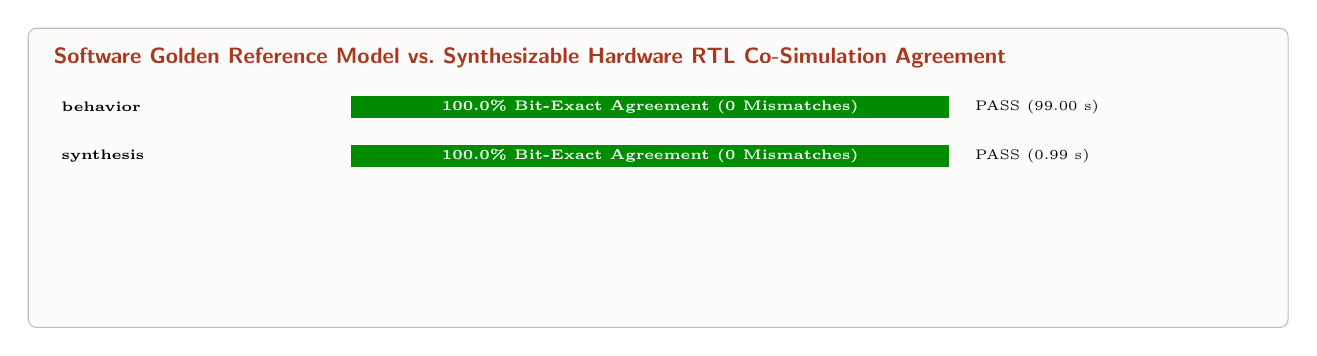
\begin{tikzpicture}[font=\scriptsize\sffamily]

\draw[draw=black!25,fill=vulcan!2,rounded corners=3pt] (-0.5,-1.85) rectangle (15.5,1.95);

\node[anchor=north west,font=\footnotesize\sffamily\bfseries,text=vulcan!90!black] at (-0.3,1.82) {Software Golden Reference Model vs.\ Synthesizable Hardware RTL Co-Simulation Agreement};

\node[anchor=west,font=\tiny\bfseries] at (-0.2,0.95) {behavior};

\fill[green!55!black] (3.6,0.81) rectangle (11.2,1.09);

\node[text=white,font=\tiny\bfseries] at (7.4,0.95) {100.0\% Bit-Exact Agreement (0 Mismatches)};

\node[anchor=west,font=\tiny] at (11.4,0.95) {PASS (99.00 s)};

\node[anchor=west,font=\tiny\bfseries] at (-0.2,0.33) {synthesis};

\fill[green!55!black] (3.6,0.19) rectangle (11.2,0.47);

\node[text=white,font=\tiny\bfseries] at (7.4,0.33) {100.0\% Bit-Exact Agreement (0 Mismatches)};

\node[anchor=west,font=\tiny] at (11.4,0.33) {PASS (0.99 s)};

\end{tikzpicture}\par

{\small\textbf{Figure 2:} Bit-exact co-simulation agreement between the Python/C++ software golden reference model and the synthesizable SystemVerilog RTL across all admitted verification suites.}\end{center}

\subsection{Unified Hardware Signoff Gates (L1 Lint, L2 Quartus STA, L3 Physical FPGA)}

{\small\renewcommand{\arraystretch}{1.18}\begin{longtable}{@{}L{0.34\textwidth}L{0.12\textwidth}L{0.46\textwidth}@{}}\toprule

\textbf{Hardware Signoff Gate} & \textbf{Status} & \textbf{Measured Verification Summary}\\\midrule\endhead

L1 Static RTL Timing \& Synthesis Lint & PASSED & Combinational div/\allowbreak{}mod hazards: 0; mixed sequential assignments (\allowbreak{}10268)\allowbreak{}: 0\\[3pt]

L2 Quartus 17.1 TimeQuest STA (\allowbreak{}Arria 10 10AX115N3F40E2SG)\allowbreak{} & PASSED & WNS\_\allowbreak{}setup =\allowbreak{} +\allowbreak{}2.929 ns,\allowbreak{} failing setup endpoints =\allowbreak{} 0,\allowbreak{} lpm\_\allowbreak{}divide errors =\allowbreak{} 0,\allowbreak{} 10268 warnings =\allowbreak{} 0\\[3pt]

\bottomrule\end{longtable}}

\begin{center}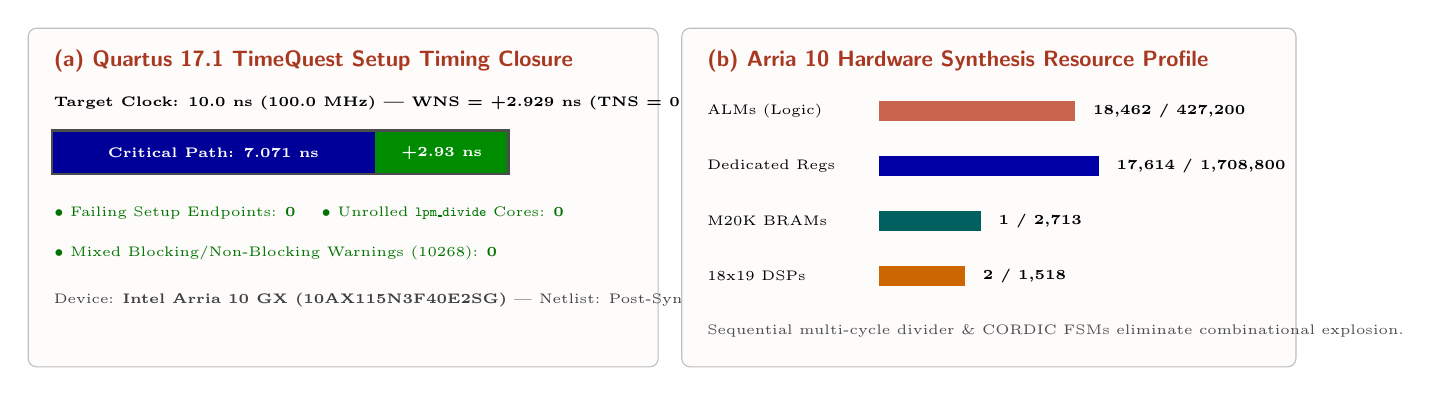
\begin{tikzpicture}[font=\scriptsize\sffamily]

\draw[draw=black!25,fill=vulcan!2,rounded corners=3pt] (-0.5,-2.1) rectangle (7.5,2.2);

\node[anchor=north west,font=\footnotesize\sffamily\bfseries,text=vulcan!90!black] at (-0.3,2.05) {(a) Quartus 17.1 TimeQuest Setup Timing Closure};

\node[anchor=west,font=\tiny\bfseries] at (-0.3,1.25) {Target Clock: 10.0 ns (100.0 MHz) | WNS = +2.929 ns (TNS = 0.000 ns)};

\fill[blue!60!black] (-0.2,0.35) rectangle (3.901,0.90);

\fill[green!55!black] (3.901,0.35) rectangle (5.600,0.90);

\draw[black!70,thick] (-0.2,0.35) rectangle (5.600,0.90);

\node[text=white,font=\tiny\bfseries] at (1.851,0.62) {Critical Path: 7.071 ns};

\node[text=white,font=\tiny\bfseries] at (4.751,0.62) {+2.93 ns};

\node[anchor=west,font=\tiny,text=green!45!black] at (-0.3,-0.15) {$\bullet$ Failing Setup Endpoints: \textbf{0} \quad $\bullet$ Unrolled \texttt{lpm\_divide} Cores: \textbf{0}};

\node[anchor=west,font=\tiny,text=green!45!black] at (-0.3,-0.65) {$\bullet$ Mixed Blocking/Non-Blocking Warnings (10268): \textbf{0}};

\node[anchor=west,font=\tiny,text=black!75] at (-0.3,-1.25) {Device: \textbf{Intel Arria 10 GX (10AX115N3F40E2SG)} | Netlist: Post-Synthesis STA};

\draw[draw=black!25,fill=vulcan!2,rounded corners=3pt] (7.8,-2.1) rectangle (15.6,2.2);

\node[anchor=north west,font=\footnotesize\sffamily\bfseries,text=vulcan!90!black] at (8.0,2.05) {(b) Arria 10 Hardware Synthesis Resource Profile};

\node[anchor=west,font=\tiny] at (8.0,1.15) {ALMs (Logic)};

\fill[vulcan!80] (10.3,1.02) rectangle (12.8,1.28);

\node[anchor=west,font=\tiny\bfseries] at (12.9,1.15) {18,462 / 427,200};

\node[anchor=west,font=\tiny] at (8.0,0.45) {Dedicated Regs};

\fill[blue!65!black] (10.3,0.32) rectangle (13.1,0.58);

\node[anchor=west,font=\tiny\bfseries] at (13.2,0.45) {17,614 / 1,708,800};

\node[anchor=west,font=\tiny] at (8.0,-0.25) {M20K BRAMs};

\fill[teal!75!black] (10.3,-0.38) rectangle (11.6,-0.12);

\node[anchor=west,font=\tiny\bfseries] at (11.7,-0.25) {1 / 2,713};

\node[anchor=west,font=\tiny] at (8.0,-0.95) {18x19 DSPs};

\fill[orange!80!black] (10.3,-1.08) rectangle (11.4,-0.82);

\node[anchor=west,font=\tiny\bfseries] at (11.5,-0.95) {2 / 1,518};

\node[anchor=west,font=\tiny,text=black!70] at (8.0,-1.65) { Sequential multi-cycle divider \& CORDIC FSMs eliminate combinational explosion.};

\end{tikzpicture}\par

{\small\textbf{Figure 3:} (a) Intel Quartus Prime 17.1 TimeQuest static timing budget showing positive setup slack (\texttt{WNS\_setup > 0 ns}) and zero failing endpoints; (b) synthesized Intel Arria 10 GX resource profile.}\end{center}

\section{Integration and use}

Compile all five rtl/\allowbreak{}*\allowbreak{}.sv files with billet\_\allowbreak{}t2\_\allowbreak{}top as the public top. T1 sources are verification inputs,\allowbreak{} not datapath dependencies. design/\allowbreak{}SPEC.md and design/\allowbreak{}ARCHITECTURE.md define public and internal contracts; tests/\allowbreak{}README.md maps requirements to retained evidence. [\allowbreak{}E001,\allowbreak{} E002,\allowbreak{} E008]\allowbreak{}


Assert rst\_\allowbreak{}n low to initialize control and diagnostics,\allowbreak{} then release it with legal configuration driven. Present natural-order samples and retain each until valid/\allowbreak{}ready acceptance. Accept exactly N inputs; use out\_\allowbreak{}ready for output backpressure. Capture exponent alongside samples and apply 2\textasciicircum{}E when restoring transform scale.


The recorded tool environment used Python 3.12.3,\allowbreak{} Icarus/\allowbreak{}vvp 12.0 and Yosys 0.33. Python verification uses only the standard library. From the project root,\allowbreak{} the behavior command is \texttt{python3 tests/\allowbreak{}verify.py --check behavior --output-dir evidence/\allowbreak{}verification/\allowbreak{}behavior}; synthesis uses \texttt{python3 tests/\allowbreak{}verify.py --check synthesis --output-dir evidence/\allowbreak{}verification/\allowbreak{}synthesis}. These commands document reproduction; no new execution is asserted by this report.


The accepted behavior result is evidence/\allowbreak{}verification/\allowbreak{}behavior/\allowbreak{}run-1745f5c6236546468a52ffa2a328cdec/\allowbreak{}result.json. Its directory retains frames.json,\allowbreak{} compatibility.json,\allowbreak{} numerical-frames.json,\allowbreak{} numerical-measurements.json,\allowbreak{} coverage,\allowbreak{} vectors,\allowbreak{} traces and subprocess receipts. Synthesis evidence is evidence/\allowbreak{}verification/\allowbreak{}synthesis/\allowbreak{},\allowbreak{} including result.json,\allowbreak{} statistics.json and netlist.json. Result receipts bind source hashes and raw execution artifacts. An existing output directory causes a fresh run child rather than replacement. [\allowbreak{}E023,\allowbreak{} E024]\allowbreak{}


\section{Limitations and acceptance boundary}

Only the five stated power-of-two lengths and fixed signed-16 sample format are supported. There is no overlapping-frame processing,\allowbreak{} automatic frame-length detection,\allowbreak{} implicit inverse normalization or public parameterization.


BFP permits at most one shift per stage and does not guarantee saturation-free arbitrary complex input. Exponent rescaling cannot recover information already lost to saturation or arithmetic truncation.


Finite simulation is not formal proof. The cumulative counter ceiling was not reached; its saturating update is supported by source inspection,\allowbreak{} while ordinary increments and reset behavior were simulated. No universal reconstruction or BFP-error bound beyond the tested conditions is established.


Generic synthesis does not establish process-node area,\allowbreak{} maximum clock frequency,\allowbreak{} timing closure,\allowbreak{} power,\allowbreak{} physical sign-off,\allowbreak{} FPGA mapping or particular SRAM inference. No board deployment or manufactured silicon was evaluated.


The retained executions establish results in the project workspace. An independent clean-directory or cross-machine reproduction was not demonstrated. Earlier design documents contain handoff-time pending language; the later source-bound results cited here establish the measured verification outcomes.


\appendix\section{Source inventory}

Production inventory: 5 Verilog/\allowbreak{}SystemVerilog files; 455 nonblank,\allowbreak{} non-comment lines. Source size is not a correctness or quality metric.

{\small\renewcommand{\arraystretch}{1.18}\begin{longtable}{@{}L{0.61\textwidth}L{0.15\textwidth}L{0.15\textwidth}@{}}\toprule

\textbf{Production file} & \textbf{Physical lines} & \textbf{Code lines}\\\midrule\endhead

rtl/\allowbreak{}billet\_\allowbreak{}t2\_\allowbreak{}bfp\_\allowbreak{}scaler.sv & 62 & 57\\[3pt]

rtl/\allowbreak{}billet\_\allowbreak{}t2\_\allowbreak{}bitrev.sv & 13 & 13\\[3pt]

rtl/\allowbreak{}billet\_\allowbreak{}t2\_\allowbreak{}butterfly.sv & 27 & 26\\[3pt]

rtl/\allowbreak{}billet\_\allowbreak{}t2\_\allowbreak{}top.sv & 221 & 216\\[3pt]

rtl/\allowbreak{}billet\_\allowbreak{}t2\_\allowbreak{}twiddle\_\allowbreak{}rom.sv & 143 & 143\\[3pt]

\bottomrule\end{longtable}}

\section{Verification record index}

{\small\renewcommand{\arraystretch}{1.18}\begin{longtable}{@{}L{0.57\textwidth}L{0.16\textwidth}L{0.17\textwidth}@{}}\toprule

\textbf{Recorded check} & \textbf{Outcome} & \textbf{Execution time (\allowbreak{}s)\allowbreak{}}\\\midrule\endhead

behavior & passed & 98.996\\[3pt]

synthesis & passed & 0.989\\[3pt]

\bottomrule\end{longtable}}

Execution times include tool and provider waiting; they are not hardware latency or model utilization.

{\small\renewcommand{\arraystretch}{1.18}\begin{longtable}{@{}L{0.12\textwidth}L{0.82\textwidth}@{}}\toprule

\textbf{Reference} & \textbf{Original project-relative record}\\\midrule\endhead

E008 & tests/\allowbreak{}README.md\\[3pt]

E012 & tests/\allowbreak{}oracle.py\\[3pt]

E014 & tests/\allowbreak{}verify.py\\[3pt]

E019 & .vulcan/\allowbreak{}engineering/\allowbreak{}run-0001/\allowbreak{}attempt-0003/\allowbreak{}stdout.log\\[3pt]

E021 & .vulcan/\allowbreak{}engineering/\allowbreak{}run-0001/\allowbreak{}attempt-0005/\allowbreak{}stdout.log\\[3pt]

E023 & .vulcan/\allowbreak{}engineering/\allowbreak{}run-0001/\allowbreak{}attempt-0007/\allowbreak{}stdout.log\\[3pt]

E024 & .vulcan/\allowbreak{}engineering/\allowbreak{}run-0001/\allowbreak{}attempt-0008/\allowbreak{}stdout.log\\[3pt]

\bottomrule\end{longtable}}

\section{Document provenance}

Engineering was independently accepted for the recorded source and evidence identity. This is not exhaustive proof, hardware deployment or physical signoff. The companion REPORT.md records the exact report approval and source manifest, and links the English/Chinese journeys containing original failures and interventions. A report number identifies a generation attempt, not a new hardware revision.

Developer attribution is explicitly supplied project metadata, not inferred affiliation or institutional endorsement.

\end{document}
